\documentclass[11pt,letterpaper]{article}

% ---------------------------------------------------------------------------
% Quantitative emergence and finite-time startup of productive polymer
% reactors: stochastic operating guarantees and certified static
% availability bounds.
%
% Author metadata: set the macros below before submission.  They are
% deliberately left blank in this version.  \CompanionAuthor is printed for
% the companion manuscripts in refs.bib; \RepositoryNote is printed under
% "Data and code availability".
% ---------------------------------------------------------------------------
\newcommand{\PaperAuthor}{}
\newcommand{\PaperAffiliation}{}
\newcommand{\PaperDate}{17 September 2026}
\newcommand{\CompanionAuthor}{Author name to be inserted}
\newcommand{\RepositoryNote}{The repository location will be supplied with the author information.}

\usepackage[T1]{fontenc}
\usepackage[utf8]{inputenc}
\usepackage{lmodern}
\usepackage{microtype}
\usepackage[letterpaper,margin=1in]{geometry}
\usepackage{amsmath,amssymb,amsthm,mathtools}
\usepackage{booktabs,array,longtable}
\usepackage{capt-of}
\usepackage{enumitem}
\usepackage{xcolor}
\usepackage{graphicx}
\usepackage{tikz}
\usetikzlibrary{arrows.meta,decorations.pathreplacing}
\usepackage[obeyspaces,spaces]{url}
\usepackage[numbers,sort&compress]{natbib}
\usepackage[colorlinks=true,linkcolor=blue!50!black,citecolor=blue!50!black,urlcolor=blue!50!black]{hyperref}
\hypersetup{pdftitle={Quantitative emergence and finite-time startup of productive polymer reactors},
  pdfkeywords={autocatalytic sets, RAF, binary polymer model, stochastic mass action, startup, martingale concentration, branching process, critical window, Lean 4}}

%% Breakable typewriter identifiers for Lean names (never inside \caption).
\DeclareUrlCommand\lean{\urlstyle{tt}}

\setlist{itemsep=2pt,topsep=3pt}
\setlength{\emergencystretch}{2em}
\graphicspath{{figures/}}

\theoremstyle{plain}
\newtheorem{theorem}{Theorem}[section]
\newtheorem{proposition}[theorem]{Proposition}
\newtheorem{lemma}[theorem]{Lemma}
\newtheorem{corollary}[theorem]{Corollary}
\theoremstyle{definition}
\newtheorem{definition}[theorem]{Definition}
\theoremstyle{remark}
\newtheorem{remark}[theorem]{Remark}
\numberwithin{equation}{section}

\newcommand{\PP}{\mathbb P}
\newcommand{\EE}{\mathbb E}
\newcommand{\cX}{\mathcal X}
\newcommand{\cR}{\mathcal R}
\newcommand{\cF}{\mathcal F}
\newcommand{\eps}{\varepsilon}
\newcommand{\ind}{\mathbf 1}
\newcommand{\dd}{\,\mathrm d}
\newcommand{\nf}{\mathrm{nf}}
\newcommand{\spc}{\mathrm{sp}}
\newcommand{\qt}{\mathrm{qt}}
\newcommand{\Vs}{V_\ast}
\newcommand{\floorstock}{(3\times10^{18})^{-1}}
\newcommand{\evid}[1]{{\normalfont\small\textsf{[}#1\textsf{]}}}

\title{Quantitative emergence and finite-time startup\\ of productive polymer reactors:\\[4pt]
\large stochastic operating guarantees and certified static availability bounds}
\author{\PaperAuthor\\[2pt]\small\PaperAffiliation}
\date{\PaperDate}

\begin{document}
\maketitle

\begin{abstract}
A reflexively autocatalytic and food-generated (RAF) set certifies that a reaction network could regenerate its catalysts from food. It supplies no deadline, stock requirement, export quota, or reliability for a finite reactor started from food alone. We study the gap between these two kinds of statement in the reversible binary polymer model with a capped Zipf catalysis source, in a fed and diluted stochastic mass-action reactor with count scale $V$. The operating requirement is a single uninterrupted trajectory that holds stock of a length-four species at times $1$, $100$ and $199$, exports more than $V/10$ nonfood monomer equivalents in each of the windows $(1,100]$ and $(100,199]$, stays in a mass corridor, and consumes at most a stated food supply. For maximum word length $n\ge4$ and integer $V\ge\max\{10^{24},10^{13}n\}$ we prove that every environment in an explicit self-catalytic witness class, with every other nonfood catalytic row unrestricted and every admitted kinetic coefficient, completes this requirement with probability at least $0.9989$. The earlier sufficient scale for the same event, model and source was $10^{60}(n+1)^2$, or about $5\times10^{49}$ after retuning. The gain comes from changing the observable: a guarded count-tail estimate supplies stock, and a one-sided logarithmic reward that discards favourable product fluctuations forces nonfood occupation and hence export. The same good event yields export above $0.42V$ over $(1,199]$, recovery of at least $1/5700$ of supplied monomer, an explicit deadline--quota--reliability trade-off, and a conditional reliability above $1-1.7\times10^{-7}$ for the original requirement. Averaging over the source gives $\Omega(2^{-n})$ success probability along the critical Zipf sequence. For the separate independent static channel fields that govern RAF emergence in the critical window, embedded dimer and three-type prefix branching processes give two-sided survival certificates, including enclosures of width below $0.006$ at openness $1/4$ and below $10^{-9}$ at openness $1/2$ in both the split and the quotient channel conventions. The finite stochastic theorem, the dimer certificates and the inverse certificate are machine-checked in Lean~4; every other statement is proved conventionally in the text and labelled as such.
\end{abstract}

\section{Introduction}\label{sec:intro}

Collectively autocatalytic sets were proposed by Kauffman \cite{kauffman1986autocatalytic,farmer1986autocatalytic} as a route by which a random chemistry could sustain itself without a single self-replicating molecule. Their combinatorial formalization, the reflexively autocatalytic and food-generated set or RAF \cite{steel2000emergence,hordijk2004detecting,steel2019autocatalytic}, is a closure statement: a set of reactions can produce all of its reactants from a food set, and each of its reactions has a catalyst so produced. In the binary polymer model RAFs appear once the mean number of reactions catalysed per molecule grows linearly with the maximum word length \cite{mossel2005random,hordijk2011required}, and heterogeneous, power-law catalysis changes both their appearance and their size \cite{hordijk2016variable,hordijk2017chasing}.

A closure statement is not an operating guarantee. It supplies no initial state, no kinetic law, no deadline, no collection rule, and no resource account. Kinetic studies of autocatalytic sets are as old as the model \cite{farmer1986autocatalytic}. Hordijk and Steel simulated molecular flow in RAF networks \cite{hordijk2012extended}; Giri and Jain separated the catalytic strength needed to maintain a large-molecule state from that needed to reach it from food \cite{giri2012origin}; Ravoni studied how composition shapes stochastic dynamics \cite{ravoni2020composition}; the stoichiometric theory of autocatalysis classifies motifs that can amplify their own species \cite{blokhuis2020universal,unterberger2022stoechiometric}; and seed-dependent activation shows why food-only initiation is a substantive restriction \cite{peng2022hierarchical}. A companion paper \cite{twowindow2026} fixed one random model in which the question can be posed exactly: the capped-Zipf binary polymer model in a fed, diluted, stochastic mass-action reactor started from food, with a two-window operating requirement on one uninterrupted trajectory. It proved a positive lower bound on success, a matching converse, and the rarity order $\Theta(2^{-n})$ along the critical Zipf sequence. Its sufficient count scale, however, was $10^{60}(n+1)^2$, or about $5\times10^{49}$ after separate retuning of its tolerances, against a necessary first-birth scale of $1.43\times10^7$.

This paper makes the operating guarantee quantitative. The model, the source, the kinetic coefficients, the preparation and the operating requirement are unchanged; only the proof changes. We ask three questions. How large must a reactor be before a specified autocatalytic witness completes the requirement with high, explicit probability? What does the same argument say about output, deadlines and material recovery? And, for the separate static probability spaces that govern the \emph{availability} of autocatalytic organizations in the critical window \cite{splitwindow2026,quotientwindow2026,shapelaw2026}, can survival probabilities at moderate openness be certified cheaply to useful precision?

\paragraph{Contributions.}
\begin{enumerate}[label=(\roman*)]
\item \emph{A finite startup theorem at a much smaller scale} (Theorem~\ref{thm:startup}). For every $n\ge4$, every Zipf exponent $\alpha>1$ and every integer $V\ge\Vs(n)=\max\{10^{24},10^{13}n\}$, every environment of the witness class, however its other nonfood catalytic rows are filled, and every admitted kinetic coefficient family, completes the original two-window requirement with probability at least $9989/10000$. Averaging over the source gives the exact witness mass times $9989/10000$, and every successful trajectory has net internal nonfood synthesis above $V/5$. \evid{Lean}
\item \emph{A mechanism.} The earlier scale was set by an absolute tolerance, about $10^{-21}$, on the selected product coordinate, squared inside a concentration estimate; helpful product births inflated a symmetric fluctuation budget. We replace it by a guarded count-tail estimate with two boundary states (Section~\ref{sec:floor}) and by a retained logarithmic reward that keeps every adverse product fluctuation and discards favourable ones (Section~\ref{sec:reward}). Section~\ref{sec:scaleset} identifies which inequality sets each of $10^{24}$ and $10^{13}n$.
\item \emph{All windows on one event} (Theorem~\ref{thm:quota}). On a single event of outer failure probability below $11/10000$, every window $(s,t]\subseteq(1,199]$ exports more than $q(t-s)V$ with $q(d)=\bigl(\tfrac{19}{10}d-82\bigr)/624-\tfrac1{20}$. \evid{Lean}
\item \emph{Consequences} (Section~\ref{sec:consequences}). Export above $263V/624>0.42V$ over $(1,199]$ and recovery above $1/5700$ of all supplied monomer; any window longer than $1756/19\approx92.4$ residence times exports more than $V/10$; the true failure budget at $\Vs$ is below $9.1\times10^{-5}$, and with a different noise level the original requirement has conditional reliability above $1-1.7\times10^{-7}$ (Proposition~\ref{prop:tradeoff}); $1600$ independent redraws of chemistry suffice for a $95\%$ screening guarantee at $n=4$; $\liminf_n2^nP_n\ge0.9989\,(6/\pi^2)^6\,9/(2\pi^2)$ along the critical sequence; and a finite-horizon continuity bound under weak food catalysis. \evid{conventional}
\item \emph{Static availability certificates} (Theorem~\ref{thm:static}). For the independent static channel fields of the critical-window law, an injectively embedded dimer forest gives $S_\nu(a)\ge1-r^{16}$ whenever $1-a+ar^4\le r$, \evid{Lean} and an embedded three-type prefix branching process gives sharper bounds that reach above $99\%$ at $a=1/4$, where the dimer construction is critical. \evid{conventional} Closed food gateways give $S_\nu(a)\le1-(1-a)^{g_\nu}$. The resulting enclosures have width below $0.006$ at $a=1/4$, below $3\times10^{-4}$ at $a=3/10$ and below $10^{-9}$ at $a=1/2$ (Table~\ref{tab:static}).
\end{enumerate}

\paragraph{Three kinds of evidence.}
Statements marked \evid{Lean} have a named declaration in a Lean~4 \cite{demoura2021lean4} and Mathlib \cite{mathlib2020} development with a strict compiler receipt (Appendix~\ref{app:formal}). Statements marked \evid{conventional} are proved in full in the text and have no separate formal export; several are short deductions from formal statements. \emph{Exact arithmetic} (rational enclosures and integer powers) is replayed by a script distributed with the source; \emph{numerical diagnostics} are labelled as such and never used as premises.

\paragraph{What is not claimed.}
The chemistry is schematic: binary words, ordered split identities, one basal scale, paired reversible coefficients, uniform washout, and a well-mixed vessel. The count scale is sufficient, not a threshold, and remains conservative by many orders of magnitude (Section~\ref{sec:physical}). The witness is a single self-catalytic ligation embedded in an arbitrary background, not a collectively autocatalytic cycle. Output is aggregate nonfood monomer effluent, not a purified or functional product. No matching upper bound, selection theorem or reliability tending to one is transferred to the new scale (Section~\ref{sec:rarity}). The static probabilities concern a different random experiment from the dynamic source and are never multiplied with dynamic probabilities.

\paragraph{Organization.}
Section~\ref{sec:models} fixes both models. Section~\ref{sec:results} states the main results. Section~\ref{sec:proof} proves the dynamic theorems, Section~\ref{sec:consequences} their consequences, and Section~\ref{sec:static} the static certificates. Section~\ref{sec:physical} discusses scale and interpretation, Section~\ref{sec:diagnostics} the diagnostics that shaped the proof, and Section~\ref{sec:discussion} open problems. Appendix~\ref{app:formal} maps statements to evidence.

\section{Two models and their probability spaces}\label{sec:models}

\begin{table}[t]
\centering\small
\begin{tabular}{@{}>{\raggedright\arraybackslash}p{.2\linewidth}>{\raggedright\arraybackslash}p{.37\linewidth}>{\raggedright\arraybackslash}p{.37\linewidth}@{}}
\toprule
 & Dynamic model (Sections~\ref{sec:dyn}--\ref{sec:proof}) & Static model (Sections~\ref{sec:staticmodel}, \ref{sec:static})\\
\midrule
Random object & catalytic rows $C_z$ with capped Zipf degrees; kinetic marks & independent Bernoulli$(a)$ openness of every channel\\
Dependence & strong within a row; rows independent & none between channel coordinates\\
Words & length at most $n$ & all finite lengths\\
State & molecule counts, continuous time & set of available word types\\
Event & two-window operating requirement by time $199$ & unbounded ordinary reversible closure\\
Parameter & Zipf exponent $\alpha>1$, count scale $V$ & openness $a\in[0,1]$\\
Probability & $\PP_\omega(F_{n,V})$ and its source average & $S_\spc(a)$, $S_\qt(a)$\\
\bottomrule
\end{tabular}
\caption{The two probability spaces. No statement below multiplies probabilities from different columns.}
\label{tab:spaces}
\end{table}

\subsection{Catalogue, source and kinetics}\label{sec:dyn}
Fix $n\ge4$. Let $\cX_n$ be the nonempty binary words of length at most $n$, and let $\cR_n$ be the ordered split identities $r=(u,v,uv)$ with $|u|,|v|\ge1$ and $|uv|\le n$. Then
\begin{equation}\label{eq:counts}
 |\cX_n|=2^{n+1}-2,\qquad R_n=|\cR_n|=\sum_{\ell=2}^n(\ell-1)2^\ell=(n-2)2^{n+1}+4 .
\end{equation}
Each identity has a ligation direction $u+v\to uv$ and a cleavage direction $uv\to u+v$. The food set is $\cF=\{0,1,00,01,10,11\}$.

\paragraph{Source.} For a real exponent $\alpha>1$, independently for each molecule $z\in\cX_n$ draw $K_z\ge1$ with $\PP(K_z=k)=k^{-\alpha}/\zeta(\alpha)$, set $D_z=\min(K_z,R_n)-1$, and given $D_z=d$ let the row $C_z\subseteq\cR_n$ of identities catalysed by $z$ be a uniformly random $d$-subset. The whole Zipf tail sits at the capped degree $R_n-1$; truncating and renormalizing would define a different source. Rows of different molecules are independent; assignments within a row are strongly dependent. Put
\begin{equation}\label{eq:marginal}
 e_\alpha=\PP(D=0)=\frac1{\zeta(\alpha)},\qquad p_{\alpha,n}=\PP(r\in C_z)=\frac{\EE D}{R_n}.
\end{equation}

\paragraph{Kinetic coefficients.} Each identity $r$ has a basal coefficient $b_r$ and each incidence $r\in C_z$ a catalytic coefficient $k_{rz}$, used in both directions, with
\begin{equation}\label{eq:box}
 \eps\le b_r\le4\eps,\qquad 4\le k_{rz}\le16,\qquad \eps=\frac1{500\,000\,000}.
\end{equation}
In the averaged model the coefficients are $b_r=\eps S_rB_r$ and $k_{rz}=4S_rH_{rz}$ with $S_r,B_r,H_{rz}$ independent and uniform on $\{1,\tfrac32,2\}$; the conditional theorems below hold pointwise on the whole box \eqref{eq:box}. An \emph{environment} $\omega$ is the rows together with the coefficients.

\paragraph{Count process.} For an integer count scale $V$, a channel with coefficient $\kappa$ and input multiplicities $s_x$, including catalyst roles, has propensity
\begin{equation}\label{eq:propensity}
 \kappa\,V^{1-m}\prod_x(N_x)_{s_x},\qquad m=\sum_xs_x,\qquad (N)_j=N(N-1)\cdots(N-j+1).
\end{equation}
The catalysed channel of $(r,z)$ has inputs $u+v+z$ and outputs $uv+z$; repeated substrate and catalyst roles are combined before the falling factorial is taken. This is an ordered-encounter coefficient convention without factorial divisors; other conventions absorb such factors into $\kappa$ \cite{anderson2011continuous}. Each food species arrives at rate $V$ and every molecule washes out at rate one per copy, so time is measured in residence times. Initially every food count is $V$ and every nonfood count is zero. On every bounded interval the process is nonexplosive and visits finitely many states, because internal reactions preserve monomer mass and feed arrivals are Poisson \cite{anderson2011continuous,ethier1986markov,norris1997markov}. $\PP_\omega$ denotes the trajectory law in a fixed environment. Normalized coordinates are $x_z=N_z/V$, the total mass $L=V^{-1}\sum_z|z|N_z$, the nonfood mass $m=V^{-1}\sum_{|z|>2}|z|N_z$, and we write
\begin{equation}\label{eq:witnesscoords}
 u=x_{00},\qquad w=x_{11},\qquad K=N_{0011}\ \ \text{(a count, not a concentration)}.
\end{equation}

\subsection{The operating requirement}\label{sec:mission}
Let $Q(s,t]$ be the monomer equivalents removed by nonfood washouts during $(s,t]$, $A(t)$ the number of food arrivals by time $t$, and $B(t)\le2A(t)$ their monomer equivalents.

\begin{definition}[Two-window requirement {\cite{twowindow2026}}]\label{def:mission}
The event $F_{n,V}$ requires, on one trajectory:
\begin{enumerate}[label=(M\arabic*)]
\item at each of the times $1$, $100$ and $199$, $L\le\tfrac{21}2$ and some species of length four has at least $V/(3\times10^{18})$ copies;
\item $Q(1,100]>V/10$ and $Q(100,199]>V/10$;
\item $L(t)\le11$ for all $0\le t\le199$, and $A(199)\le1195V$.
\end{enumerate}
\end{definition}

There is no reset, resampling of chemistry, or fresh initial law at time $100$. The stock condition is existential over length-four species; the proofs follow the single species $0011$. Figure~\ref{fig:timeline} displays the requirement.

\begin{figure}[t]
\centering
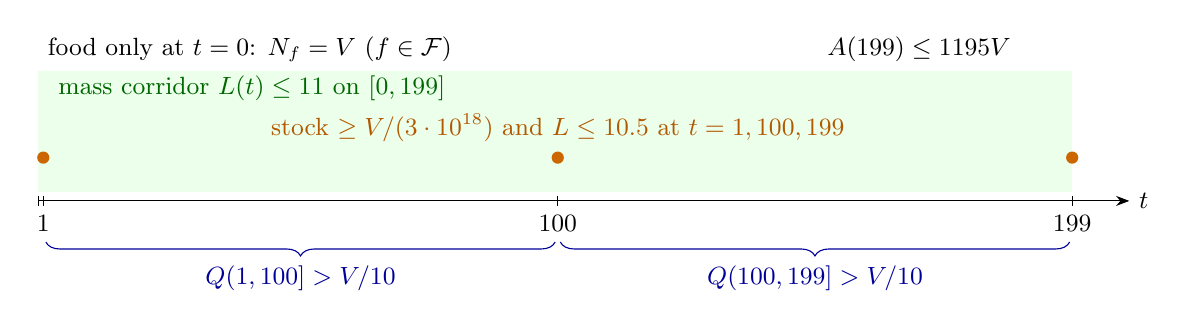
\begin{tikzpicture}[x=0.066cm,y=0.55cm,font=\small]
 \fill[green!8] (0,0.2) rectangle (199,3.0);
 \node[anchor=west,green!40!black] at (2,2.6) {mass corridor $L(t)\le11$ on $[0,199]$};
 \draw[-{Stealth}] (0,0) -- (210,0) node[right] {$t$};
 \foreach \t/\l in {1/1,100/100,199/199}{\draw (\t,0.12) -- (\t,-0.12) node[below] {\l};}
 \draw (0,0.12) -- (0,-0.12);
 \foreach \t in {1,100,199}{\fill[orange!80!black] (\t,1.0) circle (2.2pt);}
 \node[orange!70!black,anchor=south] at (100,1.15) {stock $\ge V/(3\cdot10^{18})$ and $L\le10.5$ at $t=1,100,199$};
 \draw[decorate,decoration={brace,amplitude=5pt,mirror},blue!60!black] (1.5,-0.95) -- (99.5,-0.95) node[midway,below=5pt] {$Q(1,100]>V/10$};
 \draw[decorate,decoration={brace,amplitude=5pt,mirror},blue!60!black] (100.5,-0.95) -- (198.5,-0.95) node[midway,below=5pt] {$Q(100,199]>V/10$};
 \node[anchor=west] at (150,3.5) {$A(199)\le1195V$};
 \node[anchor=west] at (0,3.5) {food only at $t=0$: $N_f=V$ ($f\in\cF$)};
\end{tikzpicture}
\caption{The single-trajectory requirement $F_{n,V}$. Stock is observed at three times; the corridor and the supply allowance cover the whole horizon, including startup from the food-only state.}
\label{fig:timeline}
\end{figure}

\begin{lemma}[Material identity {\cite{twowindow2026}}]\label{lem:material}
Let $J(t)$ be the signed nonfood monomer mass produced by internal reactions up to time $t$. On every trajectory from the food-only state,
\begin{equation}\label{eq:balance}
 m(t)V+Q(0,t]=J(t),
\end{equation}
and the total monomer supplied by time $t$ is $10V+B(t)\le10V+2A(t)$. \evid{Lean}
\end{lemma}
\begin{proof}
A food arrival does not change nonfood mass; a nonfood washout lowers it by exactly what $Q$ records; an internal reaction changes it by exactly what $J$ records. Summing over the finitely many jumps on $[0,t]$ and using $m(0)=0$ gives \eqref{eq:balance}.
\end{proof}

\subsection{The witness class}
Let $r_*=(00,11,0011)$ and let $A_n$ be the source event that all six food rows are empty and $r_*\in C_{0011}$. No other entry of $C_{0011}$ and no other nonfood row is restricted. Row independence and exchangeability within a row give
\begin{equation}\label{eq:witnessmass}
 \PP(A_n)=e_\alpha^6\,p_{\alpha,n}.
\end{equation}
On $A_n$ the product $0011$ catalyses its own formation from two distinct food dimers; this is a self-catalytic ligation witness, not a statement about collectively autocatalytic cycles.

\subsection{Static channel fields}\label{sec:staticmodel}
A \emph{split channel} is a pair $(w,i)$ with $1\le i<|w|$, representing $u+v\rightleftharpoons w$ with $|u|=i$. The \emph{quotient} convention identifies $(u,v)$ with $(v,u)$ exactly when $uv=vu$, and never identifies channels with different products \cite{quotientwindow2026}. For $\nu\in\{\spc,\qt\}$ give every channel of all finite lengths an independent Bernoulli$(a)$ open mark. The \emph{ordinary reversible closure} of an open set is the smallest set of words containing $\cF$ such that, for every open channel $u+v\rightleftharpoons uv$, availability of $u$ and $v$ implies availability of $uv$ and availability of $uv$ implies availability of $u$ and $v$. Availability is set-valued; there are no counts, rates or energies. The \emph{survival profile} is
\begin{equation}\label{eq:survival}
 S_\nu(a)=\PP_a\{\text{the closure contains words of arbitrarily large length}\}.
\end{equation}
In the independent-catalysis binary polymer model with $p_nR_n^\nu/n\to\lambda$, the probability that a RAF exists converges to $\Theta_\nu(\lambda)=S_\nu(1-e^{-\lambda})$, with $0<S_\nu(a)<1$ for $0<a<1$ \cite{splitwindow2026,quotientwindow2026}. The static field is thus the object that determines RAF \emph{availability} in the critical window; it is not the capped-Zipf source of Section~\ref{sec:dyn}.

\section{Main results}\label{sec:results}

Put $\Vs(n)=\max\{10^{24},10^{13}n\}$ and
\begin{equation}\label{eq:quota}
 q(d)=\frac{\tfrac{19}{10}d-82}{624}-\frac1{20}.
\end{equation}

\begin{theorem}[Finite startup]\label{thm:startup}
Let $n\ge4$, $\alpha>1$ and let $V\ge\Vs(n)$ be an integer.
\begin{enumerate}[label=\textup{(\alph*)}]
\item For every environment with rows in $A_n$ and coefficients in \eqref{eq:box}, $\PP_\omega(F_{n,V})\ge9989/10000$.
\item The fully averaged success probability satisfies $S_{\alpha,n,V}:=\PP(F_{n,V})\ge\tfrac{9989}{10000}\,e_\alpha^6\,p_{\alpha,n}$.
\item For every source configuration and every kinetic mark configuration, almost surely on $F_{n,V}$, $J(199)>V/5$.
\end{enumerate}
\evid{Lean: \lean{StartupMarked.startup_quantitative_resolution}}
\end{theorem}

\begin{theorem}[All windows on one event]\label{thm:quota}
Under the hypotheses of Theorem~\ref{thm:startup}\textup{(a)}, let $E_{n,V}$ be the event that $F_{n,V}$ holds and that $Q(s,t]>q(t-s)\,V$ for every $1\le s\le t\le199$. Then the outer probability of the complement of $E_{n,V}$ is less than $11/10000$.\footnote{The event quantifies over a continuum of windows. The bound is proved for the outer measure of its complement, so no separate measurability argument is needed.} Almost surely on $E_{n,V}$, $J(199)>6V/25$. \evid{Lean: \lean{StartupMarked.startup_enhanced_failure}, \lean{RandomViability.physical_enhanced_accounts}}
\end{theorem}

\begin{corollary}[Output, recovery and deadlines; conventional, from Theorem~\ref{thm:quota} and Lemma~\ref{lem:material}]\label{cor:output}
Almost surely on $E_{n,V}$:
\begin{enumerate}[label=\textup{(\alph*)}]
\item $Q(1,100]$ and $Q(100,199]$ each exceed $\tfrac{749}{6240}V>0.12\,V$;
\item $Q(1,199]>\tfrac{263}{624}V>0.42\,V$ and $J(199)>\tfrac{263}{624}V$;
\item $Q(0,199]/(10V+B(199))>263/1497600>1/5700$;
\item every window $(s,t]\subseteq(1,199]$ with $t-s>1756/19\approx92.42$ exports more than $V/10$; in particular the schedule $1,94,187$ gives two such windows, and no three disjoint windows of that length fit in $[1,199]$.
\end{enumerate}
\end{corollary}

\begin{theorem}[Static certificates]\label{thm:static}
Let $\nu\in\{\spc,\qt\}$ and $a\in[0,1]$, and put $b=1-(1-a)^2$ and $g_\spc=32$, $g_\qt=30$.
\begin{enumerate}[label=\textup{(\alph*)}]
\item \textup{(Gateways.)} $S_\nu(a)\le1-(1-a)^{g_\nu}$. \evid{Lean}
\item \textup{(Dimer forest.)} If $0\le r\le1$ and $1-a+ar^4\le r$, equivalently $a(1+r+r^2+r^3)\ge1$ when $r<1$, then $S_\nu(a)\ge1-r^{16}$. \evid{Lean}
\item \textup{(Three-type prefix process.)} If $(x,y,z)\in[0,1]^3$ satisfies, componentwise,
\begin{equation}\label{eq:threetype}
 \Bigl([(1-b)z+bx]^2,\ [(1-a)z+ax]^2,\ [1-a+ay]^2\Bigr)\le(x,y,z),
\end{equation}
then
\begin{equation}\label{eq:threelower}
 S_\spc(a)\ge1-x^4,\qquad S_\qt(a)\ge1-[(1-a)z+ax]^2\,[(1-b)z+bx]^6 .
\end{equation}
\evid{conventional}
\end{enumerate}
\end{theorem}

\begin{table}[t]
\centering\small
\begin{tabular}{@{}llll@{}}
\toprule
$a$\quad($\lambda=-\log(1-a)$) & $S_\spc(a)$ & $S_\qt(a)$ & lower-endpoint certificate\\
\midrule
$9/50$\quad($0.19845$) & $[0.4748617,\ 0.9982541]$ & $[0.4568760,\ 0.9974034]$ & three-type\\
$1/5$\quad($0.22314$) & $[0.8753628,\ 0.9992078]$ & $[0.8606719,\ 0.9987621]$ & three-type\\
$1/4$\quad($0.28768$) & $[0.9957216,\ 0.9998996]$ & $[0.9941957,\ 0.9998215]$ & three-type\\
$3/10$\quad($0.35667$) & $[0.9998233,\ 0.9999890]$ & $[0.9997091,\ 0.9999775]$ & three-type\\
 & $[0.87,\ 1-0.7^{32}]$ & $[0.87,\ 1-0.7^{30}]$ & dimer $r=\tfrac{22}{25}$ \evid{Lean}\\
$1/2$\quad($0.69315$) & $[1-200^{-4},\ 1-2^{-32}]$ & $[1-\ell_{1/2},\ 1-2^{-30}]$ & three-type\\
 & $[0.9999,\ 1-2^{-32}]$ & $[0.9999,\ 1-2^{-30}]$ & dimer $r=\tfrac{11}{20}$ \evid{Lean}\\
\bottomrule
\end{tabular}
\caption{Certified enclosures of the static survival profiles. Decimal endpoints are rounded outward from exact rational certificates; upper endpoints are the gateway bounds of Theorem~\ref{thm:static}(a). Here $\ell_{1/2}=(53/400)^2(11/160)^6$. These are rigorous enclosures, not statistical intervals. The parenthesized value is the critical-window intensity at which $\Theta_\nu(\lambda)=S_\nu(a)$.}
\label{tab:static}
\end{table}

Table~\ref{tab:static} lists certified enclosures. At $a=1/4$ both profiles exceed $99\%$, so by monotonicity of $\Theta_\nu$ \cite{splitwindow2026,quotientwindow2026} the limiting RAF probability in the independent-catalysis binary polymer model exceeds $0.9957$ (split) and $0.9941$ (quotient) for every intensity $\lambda\ge\log(4/3)$. The dimer construction alone is critical at $a=1/4$ and certifies nothing there.

\section{Proof of the finite startup theorems}\label{sec:proof}

Throughout this section $\omega$ has rows in $A_n$ and coefficients in \eqref{eq:box}, $n\ge4$, and $V\ge\Vs(n)$. The argument has four parts: a stock floor (Section~\ref{sec:floor}), a retained reward whose drift is positive when nonfood mass is small (Section~\ref{sec:reward}), a concentration bound for that reward (Section~\ref{sec:noise}), and a deterministic occupation argument (Section~\ref{sec:occupation}). Section~\ref{sec:assembly} joins them on one trajectory.

\subsection{Why the earlier scale was large}\label{sec:earlier}
The companion proof \cite{twowindow2026} compared the count process with its compensator in the concentration coordinates $(u,w,x_{0011})$ and required $|x_{0011}-\tilde x_{0011}|\le\eta_P=\floorstock/100$, one percent of the stock floor. A Freedman-type bound \cite{freedman1975tail} for this coordinate has exponent proportional to $\eta_P^2V$, so reliability forced $V\gtrsim\eta_P^{-2}\approx10^{41}$ times constants, about $5\times10^{49}$. The noise budget was symmetric: favourable product births, which help the stock requirement, were charged exactly as losses. The new proof never asks the product concentration to be close to anything. It asks for a lower count floor, which only adverse jumps can threaten, and it measures growth through a logarithm whose favourable increments may be discarded.

\subsection{Inherited envelopes and controls}
\begin{lemma}[Kinetic envelopes {\cite{twowindow2026}}]\label{lem:envelopes}
At every state with $L\le11$:
\begin{enumerate}[label=\textup{(E\arabic*)}]
\item every channel's total coefficient, basal plus catalytic contributions weighted by catalyst concentrations, is at most $C=4\eps+\tfrac{16}3m<59$;
\item the drifts of $u$ and $w$ satisfy $b_u\ge1-u-23Cu$ and $b_w\ge1-w-23Cw$;
\item every jump changes $K$ by at most two copies downward, and the copy-weighted loss rate satisfies $\sum_{\Delta K<0}|\Delta K|\,\lambda\le(1+25C)K\le1476K$;
\item every jump changes $u$ and $w$ by at most $2/V$ each, and the total rate of all channels is at most $24000V\le96000V$.
\end{enumerate}
\end{lemma}
These bounds use only the empty food rows, the coefficient box and the corridor: every active catalyst is nonfood, so its concentration is at most $m/3$; falling factorials are bounded by powers; a species is consumed by ligation in two input positions against partners of total concentration at most $11$, and by cleavage at one or three split positions. The total rate bound is the formal statement \lean{unbounded_total_rate_mass_eleven}.

\begin{lemma}[Controls]\label{lem:controls}
Let $\mathcal C$ be the event that, up to time $200$ and before the first exit from $L\le11$, the compensated total mass stays within $\tfrac14$, the compensated $u$ and $w$ stay within $10^{-5}$, the compensated export counter $Q/V$ stays within $\tfrac1{40}$, and the compensated arrival counter $A/V$ stays within $1$. Then $\PP_\omega(\mathcal C^c)\le22e^{-79}<10^{-3}$. On $\mathcal C$, for all $t\le199$: $L(t)\le10+2\cdot\tfrac14=\tfrac{21}2$; $u,w\ge\ell:=\tfrac1{1358}-2\cdot10^{-5}$; and $A(199)\le1195V$. \evid{Lean: \lean{retained_controls_uniform}, \lean{source_guard_prefix}}
\end{lemma}
\begin{proof}
The inherited exponential martingale bounds \cite{twowindow2026} give, for tolerances $d_N,d_M,d_F,d_E,d_B$ satisfying the jump margins $d_N+n/V\le\tfrac18$, $d_M+2/V\le\tfrac1{80}$, $d_F+2/V\le10^{-5}$, $d_E+n/V\le\tfrac1{40}$ and $d_B+n/V\le1$,
\[
 \PP_\omega(\mathcal C^c)\le2e^{-E_N(d_N)}+12e^{-E_C(d_M)}+4e^{-E_C(d_F)}+2e^{-E_N(d_E)}+2e^{-E_N(d_B)},
\]
with $E_N(s)=s^2V/[4n(96011\cdot200+s)]$ and $E_C(s)=s^2V/[4(96000\cdot200+2s)]$. The mass tolerance is composed from a nonfood tolerance $\tfrac18$ and six food tolerances $\tfrac1{80}$ weighted by food lengths summing to $10$. Take each $d$ equal to $0.99$ times its target. The margins hold because $n/V\le10^{-13}$ and $2/V\le2\cdot10^{-24}$. At $V=10^{24}$ and $V/n=10^{13}$ the five exponents are $1994$, $1.99\times10^{12}$, $1.28\times10^6$, $79.75$ and $1.28\times10^5$, all above $79$ and increasing in $V$ and $V/n$. Hence the bound is at most $22e^{-79}\approx1.1\times10^{-33}$.

For the deterministic consequences write the mass equation $L(t)=10+\int_0^t(10-L)\dd v+Z_L(t)$; the compensator is not constant, because dilution contributes $-L$. If $|Z_L|\le\eta$ then $e=L-10$ solves $e(t)=Z_L(t)-\int_0^te^{-(t-v)}Z_L(v)\dd v$, so $|L-10|\le\eta(2-e^{-t})\le2\eta$. For $u$, (E1)--(E2) give $b_u\ge1-1358u$, and the same comparison from $u(0)=1$ with noise at most $\eta_F$ gives $u(t)\ge\tfrac1{1358}+(1-\tfrac1{1358})e^{-1358t}-\eta_F(2-e^{-1358t})\ge\tfrac1{1358}-2\eta_F$. Arrivals have compensator $6t$. A first-exit argument removes the stopping at the corridor: the estimates preclude a first violation before time $200$.
\end{proof}

The exponent $79.75$ for the export counter is the smallest; it is where the linear term $10^{13}n$ in $\Vs(n)$ comes from (Section~\ref{sec:scaleset}).

\subsection{A guarded count floor}\label{sec:floor}
Let $\mathfrak g$ be the guard $\{L\le11,\ u\ge\ell,\ w\ge\ell\}$, and write $h=\lceil V/(3\times10^{18})\rceil$ for the stock threshold in counts.

\begin{lemma}[Power tilt]\label{lem:tilt}
Let $q=9/10$, $c=V/10^{17}$ and $1\le m_0\le V/(2\times10^{18})$ an integer with $m_0\ge10$. At every state satisfying $\mathfrak g$, the generator $\mathcal L$ of the count process satisfies
\begin{equation}\label{eq:tilt}
 \mathcal L\,q^K\le-c\,q^K+\tfrac{1558}{9}\,m_0\,q^{m_0}.
\end{equation}
\evid{Lean: \lean{physical_power_affine_generator}}
\end{lemma}
\begin{proof}
A jump changing $K$ by $d$ changes $q^K$ by $q^K(q^d-1)$. Upward jumps contribute nonpositive terms; retain only the basal forward firing of $r_*$, whose inputs $00$ and $11$ are distinct, with rate $b_{r_*}N_{00}N_{11}/V\ge\eps\ell^2V$ and weight $q-1=-\tfrac1{10}$. A loss of $d\in\{1,2\}$ copies has weight $q^{-d}-1$, and per copy lost $(q^{-1}-1)=\tfrac19<\tfrac{19}{162}=\tfrac12(q^{-2}-1)$. By (E3), $\mathcal Lq^K\le(-\tfrac1{10}\eps\ell^2V+\tfrac{19}{162}\cdot1476K)q^K=(-\imath+\tfrac{1558}9K)q^K$ with $\imath=\eps\ell^2V/10$. If $K\le m_0$, then $\tfrac{1558}9Kq^K\le\tfrac{1558}9m_0q^K$; if $K>m_0$, then $Kq^K\le m_0q^{m_0}$ because $kq^k$ decreases for $k\ge10$. In both cases \eqref{eq:tilt} follows from $c+\tfrac{1558}9m_0\le\imath$, that is, $10^{-17}+\tfrac{1558}{9}\cdot\tfrac1{2\times10^{18}}\le\eps\ell^2/10$, which holds with margin $6.08\times10^{-18}$.
\end{proof}

\begin{lemma}[Guarded tail]\label{lem:tail}
Let $m_0=\lfloor V/(2\times10^{18})\rfloor$. From any initial population, for every $t\ge1$ and every integer $j\le m_0$,
\begin{equation}\label{eq:guardedtail}
 \PP\{\mathfrak g\text{ holds at every jump state up to }t,\ K(t)\le j\}\le10\,q^{m_0-j}.
\end{equation}
\evid{Lean: \lean{source_count_tail}}
\end{lemma}
\begin{proof}
Kill the process at the first jump into a state violating $\mathfrak g$. Before killing only finitely many states are reachable on $[0,t]$, so the killed semigroup obeys Kolmogorov's equations. Put $f(t)=\EE[\ind_{\{\text{not killed by }t\}}q^{K(t)}]$. Killing removes a nonnegative payoff, so \eqref{eq:tilt} gives $f'\le-cf+\tfrac{1558}9m_0q^{m_0}$ and hence the affine envelope
\[
 f(t)\le e^{-ct}q^{K(0)}+(1-e^{-ct})\,b,\qquad b=\frac{1558\,m_0q^{m_0}}{9c}\le\frac{1558}{9}\cdot\frac{10^{17}}{2\times10^{18}}\,q^{m_0}<8.66\,q^{m_0}.
\]
The formal proof reaches the same envelope through uniformization and a Poisson mixture of the iterated finite kernel, retaining the factor $1-e^{-ct}$. For $t\ge1$, $e^{-ct}\le e^{-V/10^{17}}\le q^{m_0}$, so $f(t)\le10q^{m_0}$. On the event in \eqref{eq:guardedtail}, $q^{K(t)}\ge q^j$, and Markov's inequality gives the claim.
\end{proof}

\begin{proposition}[Uniform guarded floor]\label{prop:floor}
From any initial population, the probability that some state occupied during $[1,199]$ has $K<h$ while $\mathfrak g$ held at all earlier jump states is less than $10^{-6}$ for every real $V\ge10^{24}$. \evid{Lean: \lean{RandomViability.source_count_floor_uniform}}
\end{proposition}
\begin{proof}
A first entry into $\{K<h\}$ during $[1,199]$ either is already present at time $1$ or occurs by a jump after time $1$ from a state with $K\in\{h,h+1\}$. The second boundary state is necessary because a jump can remove two copies; Section~\ref{sec:diagnostics} gives a small chain in which omitting it undercounts crossings by three orders of magnitude. By (E3) the rate of such jumps from a guarded state is at most $1476(h+1)$. The expected number of crossings in $(1,199]$ is the integral of this rate against the occupation of $\{K\le h+1\}$ under the guard, and Lemma~\ref{lem:tail} bounds that occupation at each time. Together with the time-one term,
\[
 \PP(\text{floor failure})\le10\,q^{m_0-h+1}+1476(h+1)\cdot198\cdot10\,q^{m_0-h-1}\le10\{1+1476(h+1)\cdot198\}\,q^{m_0-h-1}.
\]
The integration uses the actual holding intervals, and divergence of jump times covers every time. Let $N=\lfloor V/10^{20}\rfloor\ge10^4$. Then $m_0-h-1\ge V/(6\times10^{18})-3\ge10N$ and $h+1\le100(N+1)$. Since $q^{10}\le\tfrac12$, the bound is at most $3\times10^8(N+1)2^{-N}$, which decreases in $N$ and is below $2.4\times10^{-20}$ already at $N=100$. The event does not assume that the guard survives; Lemma~\ref{lem:controls} supplies that.
\end{proof}

At $V\ge10^{24}$ the floor $h$ is at least $333334$ copies, which is the analytic cutoff used next.

\subsection{A retained logarithmic reward}\label{sec:reward}
Define the potential and, for each jump $N\to N'$ through channel $\mathrm{ch}$, the reward
\begin{align}
 \Phi(N)&=\log K-4H,\qquad H=(1-u)_+^2+(1-w)_+^2,\label{eq:potential}\\
 R(N,\mathrm{ch})&=\ind\{\mathrm{ch}=\mathrm{sel}\ \text{or}\ K'<K\}\,\bigl(\log K'-\log K\bigr)-4\bigl(H(N')-H(N)\bigr),\label{eq:reward}
\end{align}
where $\mathrm{sel}$ is the self-catalysed forward channel $00+11+0011\to2\cdot0011$. The reward keeps the selected self-catalytic increment and every decrease of $K$, and discards the logarithmic increments of every other favourable product birth. It keeps the full change of the food penalty. Put $R_{K_0}=\ind\{K\ge K_0\}R$ with $K_0=333334$.

\begin{lemma}[One-sided pathwise inequality]\label{lem:pathwise}
If $K>0$ at every state of a finite path segment, then $\sum R\le\Phi(N_{\rm end})-\Phi(N_{\rm start})$. \evid{Lean: \lean{retained_path_sum_le}}
\end{lemma}
\begin{proof}
Each discarded logarithmic increment is nonnegative, so each $R$ is at most the corresponding increment of $\Phi$; the increments telescope.
\end{proof}

Only the observable is thinned. The chemistry is unchanged: every favourable and adverse channel remains in the generator and in every drift estimate below.

\begin{lemma}[Drift, bracket and jump size]\label{lem:drift}
At every state with $L\le11$ and $K\ge K_0$, with $\mathcal DR=\sum_{\mathrm{ch}}\lambda_{\mathrm{ch}}R$,
\begin{align}
 \mathcal DR&\ge2-468\eps-624m-\frac{6146}{K}-\frac{3072000}{V}\ \ge\ \frac{19}{10}-624m,\label{eq:drift}\\
 \sum_{\mathrm{ch}}\lambda_{\mathrm{ch}}R^2&\le\frac{6146K}{(K-2)^2}+\frac{196608000}{V}\le\Gamma(V):=\frac{6146\cdot333334}{333332^2}+\frac{196608000}{V},\label{eq:bracket}
\end{align}
and $|R|\le2/333332+32/V<1$. At $V\ge10^{24}$, $200\,\Gamma(V)<3.6877<4$. \evid{Lean: \lean{StartupMarked.source_retained_reward_drift}, \lean{cutoff_reward_bracket}, \lean{marked_gamma_budget}}
\end{lemma}
\begin{proof}
\emph{Logarithmic part.} The selected channel has three distinct inputs, so its rate is $k\,uwK\in[4uwK,121K]$, using $k\in[4,16]$ and $uw\le(11/4)^2$ from $2u+2w\le L\le11$. For $K\ge4$ and $|d|\le2$, $\log(K+d)-\log K\ge d/K-2d^2/K^2$. The retained first moment is the selected rate minus the copy-weighted loss rate, at least $4uwK-(1+25C)K$ by (E3). The retained second moment is at most the selected rate plus twice the copy-weighted loss rate, because $d^2\le2|d|$, hence at most $121K+2\cdot1476K=3073K$. The logarithmic drift is therefore at least $4uw-1-25C-6146/K$.

\emph{Food part.} The function $h(y)=(1-y)_+^2$ has derivative bounded by $2$ in absolute value and $2$-Lipschitz derivative, so $h(y)\le h(y_0)+h'(y_0)(y-y_0)+(y-y_0)^2$. Summing over channels, $-4\sum\lambda\,\Delta H\ge8(1-u)_+b_u+8(1-w)_+b_w-4\sum\lambda(\Delta u^2+\Delta w^2)$. By (E2) and $u(1-u)_+\le\tfrac14$, $8(1-u)_+b_u\ge8(1-u)_+^2-46C$. By (E4) the Taylor term is at most $4\cdot8V^{-2}\cdot96000V=3072000/V$. The food part is therefore at least $8H-92C-3072000/V$.

\emph{Combination.} With $\alpha=(1-u)_+$ and $\beta=(1-w)_+$, $uw\ge(1-\alpha)(1-\beta)\ge1-\alpha-\beta$ and $\alpha\le2\alpha^2+\tfrac18$, so $uw\ge\tfrac34-2H$. Adding the two parts gives $\mathcal DR\ge3-8H-1-25C-6146/K+8H-92C-3072000/V$, which is \eqref{eq:drift} since $117C=468\eps+624m$. At $K\ge K_0$ and $V\ge10^{24}$ the constant part is at least $1.98156>\tfrac{19}{10}$.

\emph{Bracket and jumps.} On retained jumps $|\log(K+d)-\log K|\le|d|/(K-2)$, and every jump changes $4H$ by at most $4\cdot2\cdot(2/V+2/V)=32/V$. With $(a+b)^2\le2a^2+2b^2$, the logarithmic contribution is at most $2\cdot3073K/(K-2)^2$ and the food contribution at most $2\cdot96000V\cdot(32/V)^2$. The map $K\mapsto K/(K-2)^2$ decreases, which gives $\Gamma$. The numerical claims are exact rational comparisons.
\end{proof}

Below the cutoff the analytic reward $R_{K_0}$ vanishes, so \eqref{eq:bracket} and $|R_{K_0}|<1$ hold at every state of the corridor. The cutoff changes only the observable, never the process. On the event of Proposition~\ref{prop:floor}, $R_{K_0}=R$ at every jump after time $1$.

\subsection{Concentration of the retained reward}\label{sec:noise}
Let $Z(t)$ be the compensated cutoff reward, $\sum_{\text{jumps}\le t}R_{K_0}-\int_0^t\mathcal DR_{K_0}(N_v)\dd v$, stopped at the first exit from $L\le11$ and at time $200$.

\begin{lemma}[Exponential bound]\label{lem:noise}
For every $\delta>0$, $\PP_\omega\{\sup_{t\le200}|Z(t)|\ge\delta+1\}\le2e^{-\delta+200\Gamma(V)}$. In particular $\PP_\omega\{\sup_{t\le200}|Z(t)|\ge15\}\le2e^{-10}<99\times10^{-6}$. \evid{Lean: \lean{source_cutoff_interval_tail}, \lean{marked_noise_sharp_scalar}}
\end{lemma}
\begin{proof}
Fix $\theta\in\{1,-1\}$. Since $|\theta R_{K_0}|\le1$ and $e^y\le1+y+y^2$ for $|y|\le1$, at every corridor state $\sum\lambda(e^{\theta R_{K_0}}-1)\le\theta\mathcal DR_{K_0}+\Gamma$. Consider one holding interval from a state with total rate $\Lambda$. Its length $\tau$ is exponential with parameter $\Lambda$, and the channel is chosen with probabilities $\lambda_{\mathrm{ch}}/\Lambda$ independently of $\tau$. The one-clock identity
\[
 \EE\exp\bigl(\theta R_{K_0}-(\theta\mathcal DR_{K_0}+\Gamma)\tau\bigr)=\frac{\Lambda+\sum\lambda(e^{\theta R_{K_0}}-1)}{\Lambda+\theta\mathcal DR_{K_0}+\Gamma}\le1
\]
shows that $\exp(\theta Z-\Gamma\cdot\text{elapsed time})$, sampled at jump times and censored at the corridor exit and at time $200$, is a nonnegative supermartingale. The maximal inequality for such supermartingales, applied to the event that the prefix value $\theta Z\ge\delta$ at some jump time, gives probability at most $e^{-\delta+200\Gamma}$ \cite{freedman1975tail,bremaud1981point}; the two signs give the factor two. Inside a holding interval, $Z$ moves linearly from one prefix value to the next prefix value minus the jump $R_{K_0}$, so its absolute value exceeds the larger of the two adjacent prefix values by at most one. Taking $\delta=14$ and $200\Gamma<4$ gives the stated bound, and $e>27/10$ gives $e^{10}>2\,000\,000/99$.
\end{proof}

\subsection{Occupation forces export}\label{sec:occupation}
\begin{proposition}[Window occupation and quota]\label{prop:occupation}
Let a trajectory have positive holding times and divergent jump times, lie in the event $\mathcal C$ of Lemma~\ref{lem:controls}, avoid the floor failure of Proposition~\ref{prop:floor}, and satisfy $|Z|\le\delta+1$ on $[0,200]$. Then for all $1\le s\le t\le199$,
\begin{equation}\label{eq:occupation}
 \int_s^tm(v)\dd v>\frac{\tfrac{19}{10}(t-s)-54-2\delta}{624},\qquad \frac{Q(s,t]}V>\frac{\tfrac{19}{10}(t-s)-54-2\delta}{624}-\frac1{20}.
\end{equation}
At $\delta=14$ this is $Q(s,t]>q(t-s)V$. \evid{Lean at $\delta=14$: \lean{source_window_occupation_quota}, \lean{source_window_export_quota}}
\end{proposition}
\begin{proof}
By Lemma~\ref{lem:controls} every state occupied on $[0,199]$ satisfies $\mathfrak g$, so by Proposition~\ref{prop:floor} every state occupied on $[1,199]$ has $K\ge h\ge K_0$. Hence $R_{K_0}=R$ on the window and \eqref{eq:drift} applies to every occupied state. The compensation identity over the jumps in $(s,t]$, including the two partial holding intervals, reads
\[
 \sum_{(s,t]}R=\int_s^t\mathcal DR(N_v)\dd v+Z(t)-Z(s)\ \ge\ \tfrac{19}{10}(t-s)-624\int_s^tm\dd v-2(\delta+1).
\]
By Lemma~\ref{lem:pathwise} the left side is at most $\Phi(N_t)-\Phi(N_s)$. At time $t$, $4K\le LV\le11V$ gives $\Phi\le\log(11V/4)$. At time $s$, $K\ge V/(3\times10^{18})$ and $H\le2$ give $\Phi\ge\log(V/(3\times10^{18}))-8$. So $\Phi(N_t)-\Phi(N_s)\le\log(\tfrac{11}4\cdot3\times10^{18})+8<51.56<52$, which gives the first inequality. Each nonfood molecule of length $|z|$ washes out at rate $N_z$ and removes $|z|$ monomer equivalents, so the compensator of $Q/V$ is exactly $\int m\dd v$. Two prefix errors of at most $\tfrac1{40}$ give the second inequality.
\end{proof}

\subsection{Assembly}\label{sec:assembly}
\begin{proof}[Proof of Theorems~\ref{thm:startup} and~\ref{thm:quota}]
Let $G$ be the intersection of $\mathcal C$, the complement of the floor failure, and $\{|Z|\le15\}$. Holding times are almost surely positive, since every state has total rate at least $6V$, and jump times diverge. Almost surely on $G$, Proposition~\ref{prop:occupation} with $\delta=14$ gives $Q(s,t]>q(t-s)V$ for all windows. Here $q(99)=749/6240>1/10$, which gives (M2). Lemma~\ref{lem:controls} gives (M3) and the mass part of (M1), and Proposition~\ref{prop:floor} the stock part of (M1) at times $1$, $100$ and $199$, since each deterministic time lies in a holding interval. By the union bound, with no independence used, the outer probability of the complement of $E_{n,V}$ is less than $10^{-3}+10^{-6}+99\times10^{-6}=11/10000$. The measurable event $F_{n,V}$ therefore has probability at least $9989/10000$, which is Theorem~\ref{thm:startup}(a). Part (b) follows by integrating (a) over the mark law and over the source restricted to $A_n$, whose exact mass is \eqref{eq:witnessmass}. Part (c) and the synthesis statement of Theorem~\ref{thm:quota} follow from Lemma~\ref{lem:material}: on $F_{n,V}$, $J(199)\ge Q(1,100]+Q(100,199]>V/5$, and on $E_{n,V}$ the two quotas exceed $749V/6240$ each, and $749/3120>6/25$.
\end{proof}

\subsection{What sets the new scale}\label{sec:scaleset}
Each of the two terms of $\Vs(n)$ is set by one inequality.

\emph{The constant $10^{24}$.} The bracket \eqref{eq:bracket} needs $200\cdot6146K/(K-2)^2<4$, that is, $K\ge307304$. The drift needs only $K\ge61461$. The stock threshold of the unchanged requirement is $V/(3\times10^{18})$ copies. For the floor of Proposition~\ref{prop:floor} to reach the cutoff one needs $V\gtrsim9.2\times10^{23}$; with $K_0=333334$ this is $V>9.99999\times10^{23}$. Thus $10^{24}$ is the product of the requirement's own relative stock threshold and the variance constant of the logarithmic reward. Accepting a larger failure budget changes this little: at $99\%$ reliability one may allow $200\Gamma\le8.5$, which needs $K\ge144616$ and lowers the scale only by a factor of about $2.1$. A substantially smaller scale needs a different estimate below $3\times10^5$ copies, not a retuning of this one.

\emph{The term $10^{13}n$.} The inherited export-counter control has exponent $d_E^2V/[4n(96011\cdot200+d_E)]$ with $d_E=0.99/40$. It exceeds $79$ exactly when $V/n\ge9.906\times10^{12}$. Mass and arrival counters jump by up to $n/V$, so their exponents carry a factor $1/n$; the coordinate controls do not.

\section{Consequences}\label{sec:consequences}

\subsection{Output, recovery and deadlines}
\begin{proof}[Proof of Corollary~\ref{cor:output}]
(a) and (b) are $q(99)=749/6240$ and $q(198)=263/624$ in Theorem~\ref{thm:quota}, applied to $(1,100]$, $(100,199]$ and $(1,199]$. By \eqref{eq:balance}, $J(199)=m(199)V+Q(0,199]\ge Q(1,199]$. (c) follows from (b) and $10V+B(199)\le10V+2\cdot1195V=2400V$, since $263/(624\cdot2400)=263/1497600$. For (d), $q(d)>1/10$ exactly when $d>1756/19$. Three disjoint windows of that length need more than $277$ residence times inside $[1,199]$.
\end{proof}

The recovery ratio is a guaranteed floor in monomer equivalents, including the initial inventory. It is not a measured or typical conversion efficiency, and nothing here bounds typical recovery from above. Figure~\ref{fig:scales}(b) shows the quota function. Windows shorter than $59.58$ residence times receive no guarantee; the drift must first pay for the potential range and the endpoint noise.

\begin{figure}[t]
\centering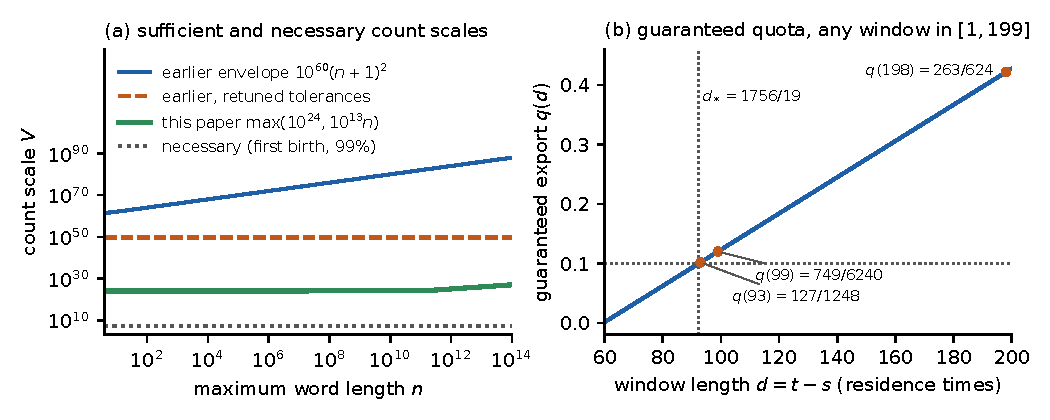
\includegraphics[width=\linewidth]{scales_quota.pdf}
\caption{(a) Sufficient count scales for the same two-window requirement: the earlier envelope, the earlier scale after unequal tolerances, and the scale proved here, together with the necessary first-birth scale for $99\%$ reliability in food-silent environments. The curves have different logical roles and are not estimates of a transition. (b) The guaranteed export $q(d)$ for any window of length $d$ inside $[1,199]$ on the single event of Theorem~\ref{thm:quota}.}
\label{fig:scales}
\end{figure}

\subsection{The true failure budget and a reliability trade-off}
The formal root rounds the three failure terms up to $10^{-3}$, $10^{-6}$ and $99\times10^{-6}$. Their proved sizes are much smaller, except for the martingale term.

\begin{proposition}[Reliability--quota trade-off]\label{prop:tradeoff}
Under the hypotheses of Theorem~\ref{thm:startup}\textup{(a)}, for every $\delta>0$, with outer probability at least $1-2e^{-\delta+3.6877}-1.1\times10^{-33}-10^{-2990}$, every window $(s,t]\subseteq(1,199]$ exports more than $\bigl[\bigl(\tfrac{19}{10}(t-s)-54-2\delta\bigr)/624-\tfrac1{20}\bigr]V$. Consequently:
\begin{enumerate}[label=\textup{(\alph*)}]
\item with $\delta=14$, the event $E_{n,V}$ has outer failure probability below $9.1\times10^{-5}$;
\item with $\delta=20$, $\PP_\omega(F_{n,V})>1-1.7\times10^{-7}$, because windows of length $99$ then still export more than $\tfrac{629}{6240}V>V/10$.
\end{enumerate}
\evid{conventional}
\end{proposition}
\begin{proof}
Lemma~\ref{lem:noise} holds for every $\delta$. Proposition~\ref{prop:occupation} is stated for general $\delta$. The controls fail with probability at most $22e^{-79}<1.1\times10^{-33}$ by the proof of Lemma~\ref{lem:controls}. The floor fails with probability at most $3\times10^8(N+1)2^{-N}$ with $N\ge10^4$, below $10^{-2990}$. At $\delta=14$, $2e^{-10}<9.081\times10^{-5}$. At $\delta=20$, $e^{20-3.6877}>1.21\times10^7$. All comparisons are exact rational computations.
\end{proof}

A larger $\delta$ buys reliability at the cost of quota and deadline. With $\delta=20$ the least window length giving $V/10$ rises from $92.42$ to $98.74$, so the original windows of length $99$ are just admissible. Reliability does not tend to one along this family at a fixed horizon: windows of length $99$ with quota $V/10$ force $\delta<20.25$, so this route cannot push the failure bound for $F_{n,V}$ below about $1.3\times10^{-7}$.

\subsection{Independent screening}\label{sec:screening}
At $n=4$ and $\alpha=2$, $R_4=68$, $e_2=6/\pi^2$ and
\[
 \EE D=67-e_2\sum_{k=1}^{67}\frac{68-k}{k^2}\approx2.5239961939,\qquad w:=e_2^6\frac{\EE D}{68}\approx0.001873651491 .
\]
Rational enclosures of $\pi$ from Machin's formula with alternating-series remainders certify $\tfrac{9989}{10000}w>L_0=187159/10^8$ and $(1-L_0)^{1600}<1/20$. If each trial independently redraws chemistry, coefficients and trajectory, the probability of at least one success in $1600$ trials is therefore above $95\%$. With the weaker reliability $0.99$ the same calculation needs $1614$ trials and gives only $0.9487$ at $1600$. Repeated runs in one sampled chemistry are conditionally independent given that chemistry but dependent after averaging, and the calculation does not apply to them. These are lower bounds for a screening design, not predicted success frequencies or recommended experiments.

\subsection{Rarity along the critical sequence}\label{sec:rarity}
Along $\alpha_n=2-2/n$, $e_{\alpha_n}\to6/\pi^2$, $\EE D/n\to9/\pi^2$ and $R_n/(n2^n)\to2$, so $2^np_{\alpha_n,n}\to9/(2\pi^2)$. Theorem~\ref{thm:startup}(b) then gives, along every integer sequence $V_n\ge\Vs(n)$,
\begin{equation}\label{eq:liminf}
 \liminf_{n\to\infty}2^n\,S_{\alpha_n,n,V_n}\ \ge\ \frac{9989}{10000}\Bigl(\frac6{\pi^2}\Bigr)^6\frac9{2\pi^2}\approx2.30\times10^{-2}.
\end{equation}
The normalized source limit and the normalized finite lower bound are formal (\lean{startup_witness_normalized_limit}, \lean{startup_normalized_source_lower}); the final conversion by $R_n/(n2^n)\to2$ is conventional. The companion converse $S\le224p+\bar r$ \cite{twowindow2026} is \emph{not} transferred. Its residual contains a term $Ce^{-cV_n/n}$, which is negligible relative to $2^{-n}$ only when $cV_n/n-n\log2\to\infty$, and a fixed ratio $V_n/n$ does not guarantee this. Failure of this transfer is not evidence that the converse fails at the new scale; it is simply not proved.

\subsection{Weak food catalysis}\label{sec:food}
The empty food rows are a genuine hypothesis. Food catalysis can initiate immediately \cite{twowindow2026}, but it also accelerates food depletion and adverse reactions. Coefficients below $4$ lie outside the box \eqref{eq:box}, so weak food catalysis defines a modified kinetic family, not another point of the original one.

\begin{proposition}[Finite-horizon continuity]\label{prop:food}
Fix an environment with rows in $A_n$ and coefficients in \eqref{eq:box}. Add, for each food $f$ and each identity $r=(u,v,uv)$, the catalysed channels $u+v+f\to uv+f$ and $uv+f\to u+v+f$ with coefficients in $[0,\eta]$ and propensities \eqref{eq:propensity}. Let $\PP^\eta_\omega$ be the resulting law. For every event $F$ determined by the path on $[0,T]$ and contained in $\{L(t)\le11,\ t\le T\}$,
\begin{equation}\label{eq:food}
 \PP^\eta_\omega(F)\ge e^{-1452\,\eta VT}\,\PP_\omega(F).
\end{equation}
In particular $\PP^\eta_\omega(F_{n,V})\ge0.9989\,e^{-1452\cdot199\,\eta V}$. \evid{conventional}
\end{proposition}
\begin{proof}
Use the random time-change representation \cite{anderson2011continuous,ethier1986markov}. Drive every original channel $k$ by an independent unit Poisson process $Y_k$ and every added channel $j$ by an independent unit Poisson process $Y'_j$. The original process $N$ solves $N(t)=N(0)+\sum_k\zeta_kY_k(\int_0^t\lambda_k(N_v)\dd v)$, and the modified process $\tilde N$ solves the same equation with the added terms. By induction over jumps, $\tilde N=N$ on $[0,T]$ on the event that no $Y'_j$ has a point in $(0,\int_0^T\lambda'_j(N_v)\dd v]$. On the corridor, $x_f\le L$ and falling factorials are bounded by powers, so
\[
 \sum_j\lambda'_j(N)\le\eta V\sum_{f\in\cF}x_f\Bigl(\sum_{(u,v)}x_ux_v+\sum_z(|z|-1)x_z\Bigr)\le\eta V\cdot11\cdot(121+11)=1452\,\eta V .
\]
The $Y'_j$ are independent of $N$. Conditional on $N$, the no-point event therefore has probability $\exp(-\sum_j\int_0^T\lambda'_j(N_v)\dd v)$, which is at least $e^{-1452\eta VT}$ on $F$. On $F$ intersected with that event, $\tilde N=N\in F$.
\end{proof}

Proposition~\ref{prop:food} establishes continuity, but at $V=10^{24}$ and $T=199$ a loss below $10^{-3}$ requires $\eta\le3.46\times10^{-33}$. It asks for no added reaction at all, whereas a macroscopic reactor tolerates many small extra reactions. A useful robustness theorem would re-derive the drift \eqref{eq:drift} with added food catalysis. On the corridor the channel coefficient envelope grows by at most $11\eta$, which suggests the replacement $2-468\eps-624m-1287\eta-6146/K-3072000/V$. But the copy-loss envelope, the food drift, the bracket and the guard survival all change, and none of these has been re-derived. We state this as an open problem, not a result.

\section{Proof of the static certificates}\label{sec:static}

\subsection{Gateways}
\begin{proof}[Proof of Theorem~\ref{thm:static}(a)]
Ligations of two food words whose product is nonfood have products of length three or four. There are $36$ ordered food pairs, $4$ of which have a food product, leaving $32$ split \emph{growth gateways}. Under the quotient, exactly the pairs $(0,00),(00,0)$ and $(1,11),(11,1)$ merge, leaving $30$. If every growth gateway is closed, then ligation from food yields food, cleavage of food yields food, and the closure equals $\cF$. The gateway coordinates are independent, which gives $S_\nu(a)\le1-(1-a)^{g_\nu}$.
\end{proof}

\subsection{Dimer forest}
\begin{proof}[Proof of Theorem~\ref{thm:static}(b)]
Consider the restricted construction that only appends a food dimer to an available word of even length. Index a branch by a sequence of dimers $(d_1,d_2,\dots,d_k)$, $k\ge2$; its edge is the channel producing $d_1\cdots d_k$ from $d_1\cdots d_{k-1}$ and $d_k$. Parsing into two-letter blocks is unique, so the product word determines the index. Distinct indices therefore have distinct products and use distinct channel coordinates, in the split model and in the quotient model alike, since the quotient never identifies channels with different products. Pulling back the independent field gives a full product law on the forest. It consists of $16$ independent four-ary marked trees, one for each first edge $d_1d_2$, and each edge is open independently with probability $a$. A tree fails by depth $k+1$ if its root edge is closed, or if it is open and all four subtrees fail by depth $k$. Hence the failure probabilities satisfy $r_0=0$ and $r_{k+1}=1-a+ar_k^4$. Monotonicity of $y\mapsto1-a+ay^4$ and $1-a+ar^4\le r$ give $r_k\le r$ by induction. Forest failure by depth $k$ has probability $r_k^{16}\le r^{16}$, and these events increase with $k$, so their union has probability at most $r^{16}$. On its complement, available words of every even length exist, because every retained step is an allowed ligation of available words through an open channel. This is unbounded closure. The full chemistry is never assumed to be a branching process; a branching process is embedded in it. Finally $1-r^4=(1-r)(1+r+r^2+r^3)$ gives the equivalent form.
\end{proof}

\subsection{The three-type prefix process}
\begin{proof}[Proof of Theorem~\ref{thm:static}(c)]
\emph{Construction.} Declare every word of length at most two \emph{reached}. A word $c$ with $|c|\ge3$ is reached if either its prefix $c'$ of length $|c|-1$ is reached and the channel $(c',\,\text{last letter})$ is open, or its prefix $c''$ of length $|c|-2$ is reached and the channel $(c'',\,\text{last two letters})$ is open. Both suffixes are food, so every reached word lies in the closure. Give a word $c$ with $|c|\ge2$ the state $(\text{reached}(c'),\text{reached}(c))\in\{0,1\}^2$, and call $c$ \emph{live} if its state is not $00$. Write $11$, $01$ and $10$ for the live states. A live word at every length implies reached words of unbounded length.

\emph{Coordinates.} The two eligible channels of $c$ both have product $c$, so channels of different words are distinct. For $|c|\ge4$ the two channels of $c$ are also distinct in the quotient model, since their factor lengths are $\{|c|-1,1\}$ and $\{|c|-2,2\}$. For $|c|=3$, $c=\alpha\beta\gamma$, the quotient identifies $(\alpha\beta,\gamma)$ with $(\alpha,\beta\gamma)$ exactly when $\alpha=\beta=\gamma$, that is, for $000$ and $111$. All channels of words at one length are disjoint from those at every other length.

\emph{Branching structure.} Given the states of all words of length at most $\ell$, the states of the words of length $\ell+1$ are determined by those states and by fresh coordinates, distinct for distinct children. Each child $c=c'\gamma$ has state $(\text{reached}(c'),\text{reached}(c))$, and $\text{reached}(c)$ depends only on the state of $c'$ and the coordinates of $c$. Hence, for $|c'|\ge3$ in both models and for $|c'|\ge2$ in the split model, the live words form a multitype Galton--Watson process \cite{harris1963branching,athreya1972branching} in which each word has two children with independent states given its own:
\begin{itemize}
\item from $11$, a child is reached with probability $b=1-(1-a)^2$ (state $11$), else it has state $10$;
\item from $01$, a child is reached with probability $a$ (state $11$), else state $10$;
\item from $10$, a child is reached with probability $a$ through the dimer channel (state $01$), else it is dead ($00$), and dead words have only dead descendants.
\end{itemize}

\emph{Extinction.} Let $x_k,y_k,z_k$ be the probabilities that no live word exists $k$ generations below a word of state $11$, $01$ or $10$. Then $(x_0,y_0,z_0)=0$ and $(x_{k+1},y_{k+1},z_{k+1})$ is the left side of \eqref{eq:threetype} evaluated at $(x_k,y_k,z_k)$, since the two children are independent. This map is coordinatewise nondecreasing, so a supersolution $(x,y,z)$ bounds every iterate. Extinction by depth $k$ increases to extinction, whose probability is therefore at most $x$, $y$ or $z$.

\emph{Initial layers.} In the split model the four dimers have state $11$ and independent subtrees, so $S_\spc(a)\ge1-x^4$. In the quotient model start one layer later. The eight words of length three have independent coordinates. Each of the six words other than $000$ and $111$ is reached with probability $b$, and $000$ and $111$ with probability $a$, because their two descriptions are one coordinate. A reached word has state $11$ and an unreached one state $10$, since its dimer parent is reached. The length-three subtrees are independent and at depth at least four the recursion is exact, which gives $S_\qt(a)\ge1-[(1-a)z+ax]^2[(1-b)z+bx]^6$.
\end{proof}

The literal restricted construction was also enumerated exactly at $a=3/10$ to depth two below a dimer: all $2^{12}$ split assignments and all $2^{11}$ quotient assignments, including the merged coordinate of $000$. The enumerated extinction probabilities agree with the recursion. This is a check of the bookkeeping, not part of the proof.

\subsection{Certificates, inverse design and construction thresholds}\label{sec:certs}
A supersolution is found numerically, perturbed along the Perron vector of the Jacobian at the numerical fixed point, rounded up to denominators $10^{12}$, and then verified exactly in rational arithmetic. No floating-point fixed point is used as a certificate. Table~\ref{tab:static} lists five openness values, Figure~\ref{fig:static} shows eighty-five certified points, and Table~\ref{tab:inverse} gives inverse design values. At $a=1/2$ the short vector $(1/200,9/500,13/50)$ has minimum slack $7/25600$ and gives widths below $4\times10^{-10}$ (split) and $10^{-9}$ (quotient). At $a=3/10$ the dimer candidates $r=0.87$ and $0.879$ fail the supersolution test while $r=22/25$ passes; failure of a candidate says nothing about the profile.

\begin{figure}[t]
\centering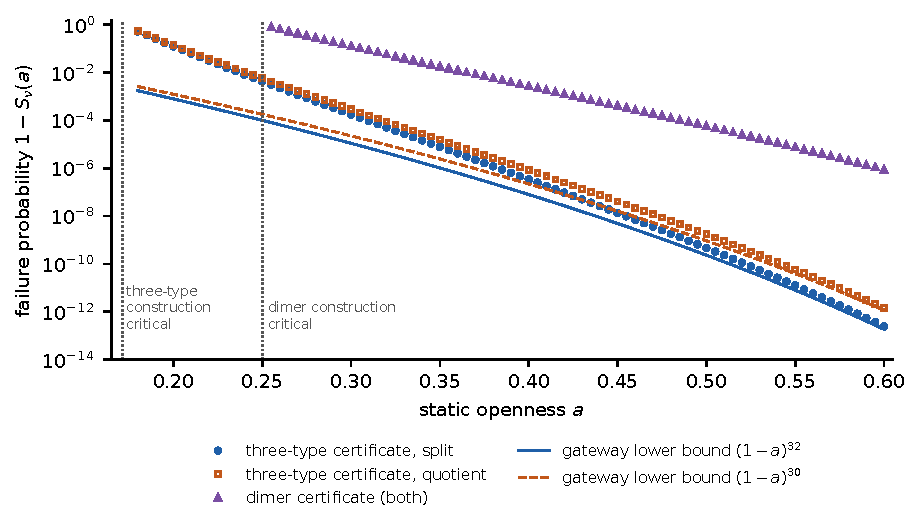
\includegraphics[width=.9\linewidth]{static_certificates.pdf}
\caption{Certified bounds on the failure probability $1-S_\nu(a)$. Markers are upper bounds from exact three-type and dimer certificates at each plotted openness; lines are the gateway lower bounds. The vertical lines mark where each restricted construction becomes critical; neither is a threshold of the static model, whose survival is positive for every $a>0$.}
\label{fig:static}
\end{figure}

\begin{table}[t]
\centering\small
\begin{tabular}{@{}lccccc@{}}
\toprule
Target survival & \multicolumn{2}{c}{Necessary: $a$ exceeds} & \multicolumn{3}{c}{Sufficient: $a\ge$}\\
\cmidrule(lr){2-3}\cmidrule(lr){4-6}
 & split & quotient & dimer (both) & three-type, split & three-type, quotient\\
\midrule
$99\%$ & $0.1340$ & $0.1423$ & $0.3658$ & $0.2371$ & $0.2412$\\
$99.9\%$ & $0.1941$ & $0.2056$ & $0.4265$ & $0.2726$ & $0.2792$\\
$99.99\%$ & $0.2501$ & $0.2643$ & $0.4863$ & $0.3091$ & $0.3183$\\
$99.9999\%$ & $0.3506$ & $0.3690$ & $0.5972$ & $0.3830$ & $0.3970$\\
\bottomrule
\end{tabular}
\caption{Inverse design for the static profiles. A necessary entry $a_0$ satisfies $(1-a_0)^{g_\nu}>1-{}$target exactly, so survival at openness $a_0$ is below the target. A sufficient entry carries an exact certificate at that openness. These values bracket a target openness without locating any transition.}
\label{tab:inverse}
\end{table}

The dimer construction has mean offspring $4a$ and is critical at $a=1/4$. The three-type construction has mean matrix with rows $(2b,0,2(1-b))$, $(2a,0,2(1-a))$ and $(0,2a,0)$, whose spectral radius crosses one at $a\approx0.1713509469$. Below these values the constructions certify nothing. This is a limitation of the embedded subnetworks, not a threshold of $S_\nu$, which is positive for every $a>0$ \cite{splitwindow2026,quotientwindow2026}. The companion effective-approximation paper gives an explicit rational evaluator for $S_\nu$ at every openness, with an exponentially large cap at moderate $a$ \cite{shapelaw2026}. The certificates here complement it: they are inexpensive and precise from $a\approx0.2$ upward and silent below.

\section{Scale and physical interpretation}\label{sec:physical}

\paragraph{Dimensions.} For a physical volume $\Omega$ in litres, a concentration scale $c_*$ in mol/L and a residence time $\tau$,
\begin{equation}\label{eq:units}
 V=N_A\Omega c_*,\qquad t_{\rm phys}=\tau t,\qquad k_{\rm phys}=\frac{\kappa}{\tau\,c_*^{\,m-1}},
\end{equation}
where $m$ counts catalyst input roles and $N_A=6.02214076\times10^{23}\,\mathrm{mol}^{-1}$ exactly \cite{bipm2019si}. Table~\ref{tab:units} gives the volume at $V=10^{24}$. Each food species has initial concentration $c_*$, so the total initial molecular concentration is $6c_*$. A normalized window export of $0.12$ is about $0.199$ mol of monomer equivalents, and the whole-horizon guarantee $263/624$ about $0.700$ mol. Meanwhile the guaranteed selected stock is only $333334$ molecules, a concentration of $3.3\times10^{-19}c_*$. The requirement controls quantities on very different scales, and the export must not be read as the concentration of the selected tetramer. With $\tau=1$ h the horizon is $199$ h. Changing $c_*$ while keeping the dimensionless box fixed changes the physical rate constants, and equal paired dimensionless coefficients have different physical units when their molecularities differ.

\begin{table}[t]
\centering\small
\begin{tabular}{@{}lccc@{}}
\toprule
$c_*$ & $1$ M & $1$ mM & $1$ $\mu$M\\
\midrule
$\Omega$ at $V=10^{24}$ & $1.66054$ L & $1660.54$ L & $1.66054\times10^6$ L\\
\bottomrule
\end{tabular}
\caption{Dimensional reading of the count scale. This is a conversion, not a feasible design; the dilute mass-action assumptions are not validated at these concentrations.}
\label{tab:units}
\end{table}

\paragraph{Necessary versus sufficient.} In every food-silent environment the mission probability is at most $1-\exp[-(484/3)\eps V]$ \cite{twowindow2026}, so $99\%$ reliability needs $V\ge14\,272\,222$, about $23.7$ pL at $1\,\mu$M. The sufficient scale $10^{24}$ covers far more than first birth: stock persistence, food and mass control, and two export windows. The gap of seventeen orders of magnitude is unresolved sharpness. Neither endpoint is an observed transition, and Section~\ref{sec:scaleset} shows that closing the gap requires an estimate below about $3\times10^5$ copies of the product.

\paragraph{What transfers.} The transferable object is a proof contract for a stochastic operating question: (1) specify the chemistry or its source, the initial counts and the coefficient uncertainty; (2) specify stock, output, deadlines, feed and losses as one trajectory event; (3) separate the probability of acquiring the chemistry from the probability of completing the task given it; (4) choose an observable whose fluctuations are exactly the ways the task can fail, and check whether favourable reactions inflate a symmetric noise estimate; (5) verify the count floor, retained drift, bracket, export and mass inequalities for the actual generator; (6) report conditional and averaged guarantees with their units and their unvalidated assumptions. Monomer conservation is a material balance and not a thermodynamic statement; free-energy supply and dissipation need their own accounting \cite{rao2016nonequilibrium}. No assay threshold, clinical risk estimate or reactor design follows from the present abstract model.

\section{Diagnostics that shaped the proof}\label{sec:diagnostics}

The following small computations were run to test proposed inequalities. None is a premise of any theorem.

\paragraph{Symmetric versus retained variance.} At $n=8$, $V=10^{24}$, all food counts equal to $V$, $K=333334$, other nonfood counts zero, and the full catalogue of basal channels, feed and washout, the literal generator gives a retained bracket $\sum\lambda R^2\approx1.50\times10^{-5}$. The logarithmic increments of favourable non-selected product births have $\sum\lambda(\Delta\log K)^2\approx1.80\times10^4$. A symmetric fluctuation estimate for $\log K$ is dominated by reactions that help the requirement; discarding them costs only a one-sided inequality (Lemma~\ref{lem:pathwise}). Across ten fixtures at $n\in\{4,8\}$, including hostile trimer backgrounds with $m=10$ and repeated-role double losses, every envelope of Lemma~\ref{lem:drift} held.

\paragraph{Two boundary states.} In a chain on $\{0,\dots,30\}$ with immigration rate $8$, loss $k\to k-2$ at rate $k/2$ ($k\ge2$) and $1\to0$ at rate $1$, and threshold $K<4$ from $K=5$, the probability of crossing by time $0.01$ is $0.02374$. The expected number of crossings from state $4$ alone is $1.36\times10^{-5}$, so omitting the second boundary state $h+1$ gives an invalid bound. Including it gives $0.02375$.

\paragraph{Affine renewal.} The naive envelope $\EE f\le e^{-ct}f+b$, iterated over renewal steps, charges $b$ repeatedly and is false: in a small finite-kernel test with $b=0.2$ and $f=0$ the true value was $0.20494$. The retained form $e^{-ct}f+(1-e^{-ct})b$ of Lemma~\ref{lem:tail} is what the formal recursion uses.

\paragraph{Logarithm Lipschitz constant.} With the denominator $K-2$ the bracket gives $200\Gamma\approx3.688$. A gratuitous factor two in the logarithm's Lipschitz constant would exceed the budget $4$ that makes $\delta=14$ yield $2e^{-10}$.

\section{Discussion}\label{sec:discussion}

\paragraph{Availability, initiation and operation.} Three requirements are routinely conflated when a structural autocatalytic certificate is read as a prediction. \emph{Availability} of an autocatalytic organization is a source or static-field event: probability $\Theta_\nu(\lambda)$ in the independent critical window, certified here above $99\%$ at $\lambda\ge\log(4/3)$, and $e_\alpha^6p_{\alpha,n}=\Theta(2^{-n})$ for the witness class of the capped Zipf source. \emph{Initiation} in a food-silent environment is a first-passage event with hazard at most $(484/3)\eps V$. \emph{Operation}, a trajectory event with stock, deadlines, quotas and a supply account, holds with probability at least $0.9989$ given the witness at $V\ge\Vs(n)$. The three probabilities live on different spaces and are reported separately.

\paragraph{Why the observable matters.} The improvement from $5\times10^{49}$ to $10^{24}$ did not come from a stronger concentration inequality. It came from deriving the observable from the failure event. Stock can only be lost through adverse jumps, and growth need only be certified from below. A count-tail estimate and a one-sided reward encode exactly these facts, and the fluctuation budget stops paying for favourable reactions.

\paragraph{Open problems.}
(1) \emph{Smaller scale.} Below $3\times10^5$ copies the logarithmic bracket fails. A seed-to-established-stock comparison with relative error, jointly with food retention, is needed to approach the necessary scale.
(2) \emph{Weak food catalysis.} Re-derive the loss envelope, drift, bracket and guard survival with added food-catalysed channels of strength $\eta$, and find the largest $\eta$ for which the conclusion of Theorem~\ref{thm:startup} survives at fixed reliability.
(3) \emph{Converse at the new scale.} Prove $S_{\alpha_n,n,V_n}=O(2^{-n})$ and singleton selection along sequences with $V_n=O(n)$, or show that they fail.
(4) \emph{Collective witnesses.} Replace the self-catalytic ligation by a mutually catalytic pair or cycle; the floor and reward arguments then need multi-species potentials.
(5) \emph{Low openness.} Certify $S_\nu(a)$ to useful precision below $a\approx0.17$, where both embedded constructions are subcritical.
(6) \emph{Formalization.} The three-type static bound and the trade-off of Proposition~\ref{prop:tradeoff} are conventional; formalizing them requires a finite-depth joint-law lemma for the live-prefix states and a general-$\delta$ occupation statement.

\paragraph{Data and code availability.}
\RepositoryNote{} The source package contains this manuscript, its bibliography, the figure script, and an exact-arithmetic script that replays every printed number, certifies every static point and enumerates the literal prefix construction. It also contains the diagnostic scripts and their outputs, and the verification manifest of the formal development (Appendix~\ref{app:formal}).

\appendix

\section{Formal scope and reproducibility}\label{app:formal}

The formal development is a single Lean~4 project pinned to \texttt{leanprover/lean4:v4.30.0} with a pinned Mathlib manifest. Verification is performed through a wrapper that treats every warning as an error and records a strict receipt with the source hash. Explicit declaration probes report only the standard axioms \texttt{propext}, \texttt{Classical.choice} and \texttt{Quot.sound}; no admitted proof or additional axiom occurs. The physical process is the literal continuous-time jump law with the propensities \eqref{eq:propensity}, all channels present, and the source is the capped Zipf configuration weight with the uniform finite mark law. Table~\ref{tab:formal} maps statements to evidence. Declarations live under \path{proofs/StartupMarked/}, \path{proofs/StartupCount/}, \path{proofs/PracticalCriticalWindow/}, \path{proofs/RepeatedFunction/} and \path{proofs/RandomViability/}.

{\small
\begin{longtable}{@{}>{\raggedright\arraybackslash}p{.3\linewidth}>{\raggedright\arraybackslash}p{.12\linewidth}>{\raggedright\arraybackslash}p{.52\linewidth}@{}}
\caption{Statements of this paper and their evidence.}\label{tab:formal}\\
\toprule
Statement & Evidence & Declarations or remark\\
\midrule
\endfirsthead
\toprule
Statement & Evidence & Declarations or remark\\
\midrule
\endhead
Theorem~\ref{thm:startup} & Lean & \lean{StartupMarked.startup_quantitative_resolution} (root; uses $9989/10000$, the exact witness mass and the signed synthesis account)\\
Theorem~\ref{thm:quota} & Lean & \lean{StartupMarked.startup_enhanced_failure}, \lean{StartupMarked.source_window_export_quota}, \lean{RandomViability.physical_enhanced_accounts}\\
Lemma~\ref{lem:material} & Lean & \lean{physical_mission_accounts} and the companion identity \lean{actual_net_synthesis_identity}\\
Lemma~\ref{lem:envelopes} & inherited & companion derivation \cite{twowindow2026}; \lean{unbounded_total_rate_mass_eleven}, \lean{physical_crossing_rate_le}\\
Lemma~\ref{lem:controls} & Lean & \lean{retained_controls_failure}, \lean{retained_controls_uniform}, \lean{retained_exponents}, \lean{physical_mass_localization}, \lean{physical_food_floor_from_noise}, \lean{source_guard_prefix}\\
Lemma~\ref{lem:tilt} & Lean & \lean{physical_power_generator}, \lean{physical_power_affine_generator}, \lean{affine_power_envelope}\\
Lemma~\ref{lem:tail} & Lean & \lean{poissonized_affine_generator}, \lean{source_count_terminal_bound}, \lean{source_count_tail}\\
Proposition~\ref{prop:floor} & Lean & \lean{source_count_crossing_bound}, \lean{source_count_floor_coarse}, \lean{count_rounding_bounds}, \lean{uniform_crossing_scalar_certificate}, \lean{source_count_floor_uniform}\\
Lemma~\ref{lem:pathwise} & Lean & \lean{retained_reward_le_potential_increment}, \lean{retained_path_sum_le}\\
Lemma~\ref{lem:drift} & Lean & \lean{source_retained_reward_drift}, \lean{source_retained_reward_bracket}, \lean{cutoff_reward_bracket}, \lean{cutoff_reward_abs}, \lean{marked_drift_margin}, \lean{marked_gamma_budget}, \lean{marked_jump_budget}\\
Lemma~\ref{lem:noise} & Lean & \lean{gamma_reward_crossing_tail}, \lean{gamma_reward_two_sided_tail}, \lean{gamma_reward_interval_tail} (general $\delta$), \lean{source_cutoff_interval_tail} ($\delta=14$), \lean{marked_noise_sharp_scalar}\\
Proposition~\ref{prop:occupation} & Lean at $\delta=14$ & \lean{source_window_occupation_quota}, \lean{source_window_export_quota}; general $\delta$ conventional\\
Section~\ref{sec:assembly} & Lean & \lean{startup_enhanced_mission}, \lean{startup_mission_failure}, \lean{startup_concrete_success}, \lean{startup_fully_averaged_lower}\\
Section~\ref{sec:scaleset} & arithmetic & exact thresholds $307304$, $61461$, $9.906\times10^{12}$\\
Corollary~\ref{cor:output} & conventional & from Theorem~\ref{thm:quota}; the $6/25$ synthesis bound is Lean\\
Proposition~\ref{prop:tradeoff} & conventional & general-$\delta$ tail is Lean; control and floor sizes from their formal proofs\\
Section~\ref{sec:screening} & arithmetic & Machin enclosure; integer powers\\
Equation~\eqref{eq:liminf} & Lean + conv. & \lean{startup_witness_normalized_limit}, \lean{startup_normalized_source_lower}; final conversion conventional\\
Proposition~\ref{prop:food} & conventional & random time-change coupling\\
Theorem~\ref{thm:static}(a) & Lean & \lean{split_gateway_upper}, \lean{quotient_gateway_upper}\\
Theorem~\ref{thm:static}(b) & Lean & \lean{dimerPrefixIndex_injective}, \lean{sourceForest_law}, \lean{appendTree_generation}, \lean{dimer_split_survival_lower}, \lean{dimer_quotient_survival_lower}, \lean{inverse_source_certificate}, \lean{half_open_profile_real_intervals}, \lean{three_tenths_profile_real_intervals}\\
Theorem~\ref{thm:static}(c) & conventional & proof in Section~\ref{sec:static}; exact enumeration check to depth two\\
Tables~\ref{tab:static}, \ref{tab:inverse}; Figure~\ref{fig:static} & arithmetic & exact rational supersolutions\\
Section~\ref{sec:diagnostics} & numerical & diagnostics only\\
\bottomrule
\end{longtable}
}

\paragraph{Reproduction.} The script \texttt{check\_paper.py} replays every printed number in exact rational arithmetic in about twenty seconds. It checks the floor constants and rounding, the drift, bracket and jump constants, the control exponents, the occupation and quota algebra, the budget and its sharpening, the screening enclosure, the necessary scale, the weak-food constant and the unit conversions. It also searches for, rounds and exactly verifies every static certificate, computes the inverse table and the construction thresholds, and enumerates the literal prefix construction. The script \texttt{make\_figures.py} draws both figures from these certified values. Formal verification uses the repository wrapper with an explicit declaration, for example \lean{StartupMarked.startup_quantitative_resolution} in \path{proofs/StartupMarked/Resolution.lean}. The source hashes of the eight principal files match the verification manifest distributed with the package; no dependency update is performed.

\bibliographystyle{plainnat}
\bibliography{refs}

\end{document}
